% Chapter 1

\chapter{Introduzione} % Chapter title

\label{ch:introduction} % For referencing the chapter elsewhere, use \autoref{ch:introduction} 

Con il termine \textit{frana} si indicano tutti i fenomeni di movimento di terreno, come ad esempio caduta di rocce e  scivolamento di detriti superficiali, lungo un pendio.
La forza di gravità, a cui è soggetta la massa di terreno, è sicuramente la causa scatenante più importante ma non è l'unica. Una frana avviene nel momento in cui un pendio passa da una condizione di stabilità ad una di instabilità.
Tale passaggio di stato è causato da diversi fattori i quali possono contribuire contemporaneamente o singolarmente.
Tra le cause naturali sono evidenziati le seguenti:

\begin{enumerate}
	\item pressione di acqua sotterranea (acqua piana) che agisce per destabilizzare la pendenza;
	\item assenza di vegetazione (dovuta ad esempio ad un incendio);
	\item erosione della punta di un pendio;
	\item indebolimento di un pendio a causa di piogge pesanti o scioglimento di ghiacci/neve;
	\item terremoti che aggiungono carichi a pendenze già poco stabili.
\end{enumerate}
Il fenomeno delle frane è aggravato inoltre da fattori riconducibili alle attività umane come:
\begin{enumerate}
	\item deforestazioni e costruzioni che destabilizzano i pendii;
	\item sterri che alterano la forma dei pendii e che quindi posso aggiungere nuovi carichi.
\end{enumerate}
Una frana generalmente è caratterizzata dal tipo di materiale movimentato (ad esempio materiale roccioso o semplicemente detriti superficiali) e dal tipo di movimento che il materiale segue. Queste due caratteristiche principali vengono poi integrate considerando anche altri aspetti come la velocità e l'entità del movimento.
In base al comportamento della frana possiamo quindi avere la seguente classificazione: 
\begin{enumerate}
	\item \textbf{Frane di crollo:} massa che si stacca da un versante molto acclive e che, successivamente, si muove per caduta libera, rimbalzo, rotolamento. Il distacco può avvenire per rottura di taglio o di trazione della roccia (Figura \ref{crollo}).
	\item \textbf{Frane da ribaltamento:} rotazione in avanti, verso l'esterno del versante, di una massa di terra o roccia, intorno ad un punto situato al di sotto del baricentro della massa spostata (Figura \ref{ribaltamento}).
	\item \textbf{Frana da scivolamento planare:} movimento verso la base del versante di una massa di terra o roccia che avviene per deformazioni di taglio lungo una o più superfici o entro uno spessore limitato di materiale (Figura \ref{scivolamento}).
	\item \textbf{Frana da colata o colamento:} movimento distribuito in maniera continua all'interno della massa spostata. Le superfici di taglio, se presenti, sono multiple e spesso temporanee. La distribuzione delle velocità nella massa
	spostata è analoga a quella all'interno di un fluido viscoso  (Figura \ref{colata}).
\end{enumerate}

\begin{figure}[h]
	\hspace{0.1\linewidth}
	\begin{minipage}[t]{0.35\linewidth}
		\centering
		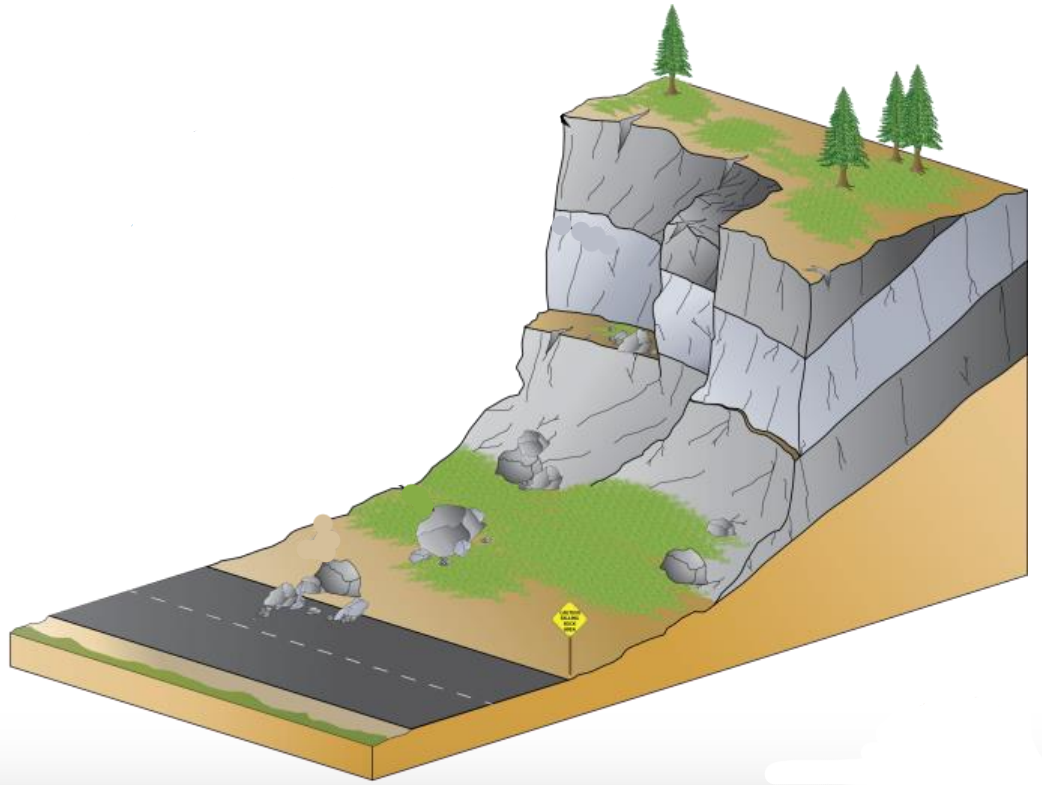
\includegraphics[width=\textwidth]{images/crollo}
		\caption{Frana di crollo. I massi che si staccano dalla cima rotolano lungo il pendio e arrivano a valle. }
		\label{crollo}
	\end{minipage}
	\hspace{0.1\linewidth}
	\begin{minipage}[t]{0.35\linewidth}
		\centering
		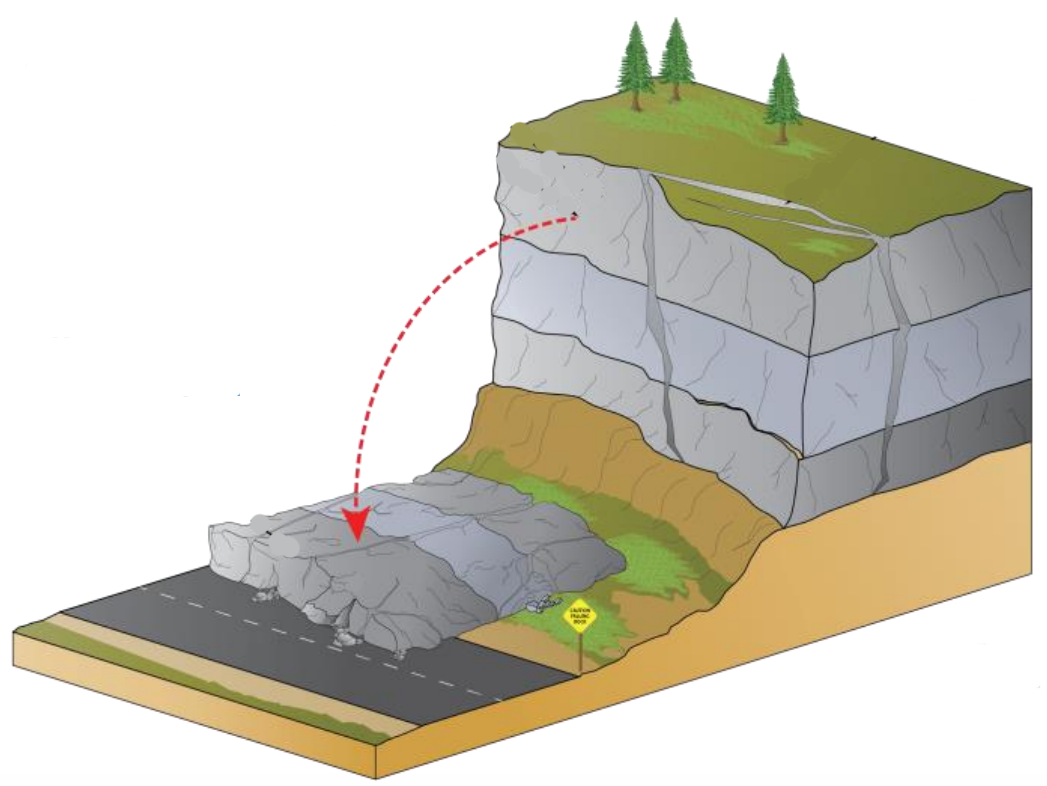
\includegraphics[width=\textwidth]{images/Ribaltamento}
		\caption{Frana di ribaltamento. Un'intera parete rocciosa si distacca dal pendio.}
		\label{ribaltamento}
	\end{minipage}
\end{figure}

\begin{figure}[h]
	\hspace{0.1\linewidth}
	\begin{minipage}[t]{0.35\linewidth}
		\centering
		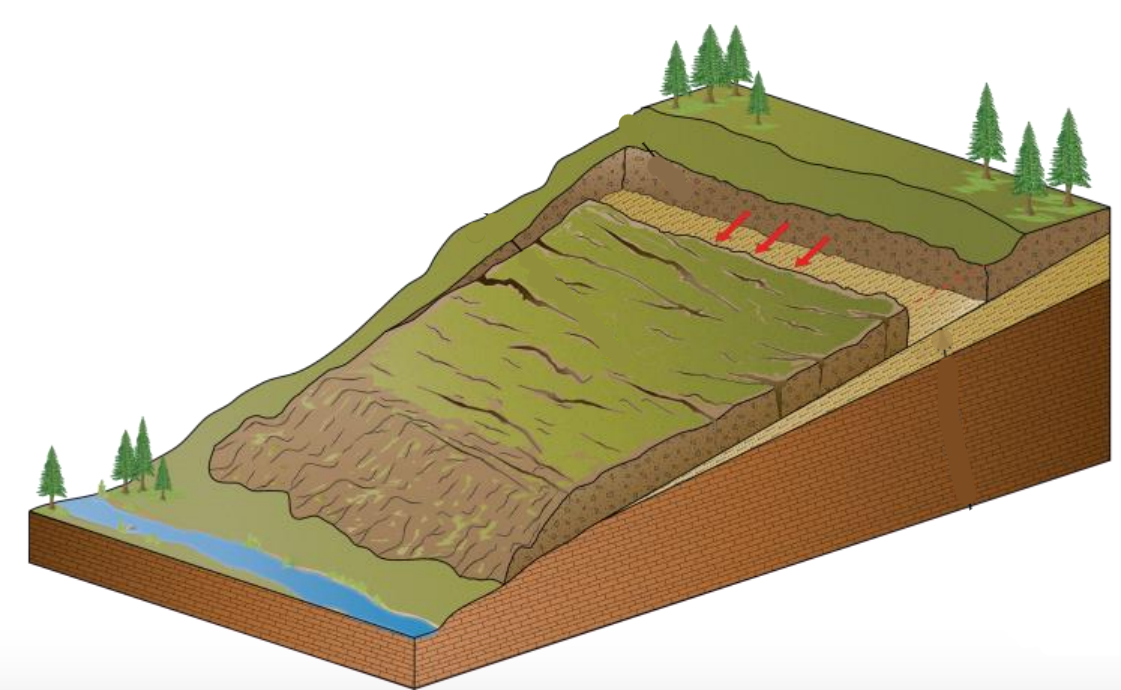
\includegraphics[width=\textwidth]{images/Scivolamento_planare}
		\caption{Frana da scivolamento planare. Un'area di terreno intera scivola verso la valle.}
		\label{scivolamento}
	\end{minipage}
	\hspace{0.1\linewidth}
	\begin{minipage}[t]{0.35\linewidth}
		\centering
		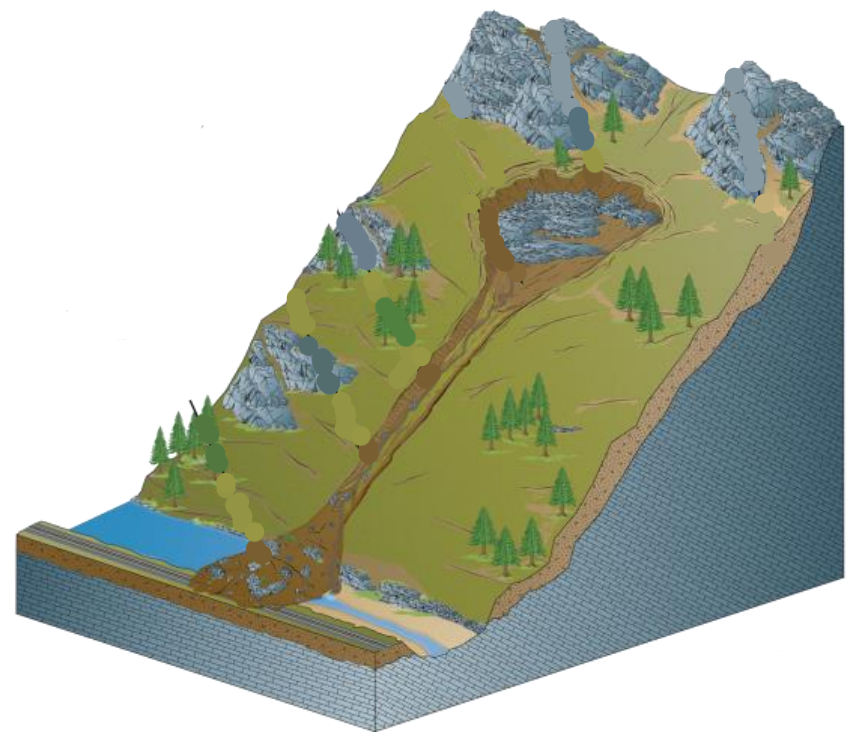
\includegraphics[width=\textwidth]{images/colata}
		\caption{Frana da colata. I detriti scivolano verso la valle formando un corridoio. }
		\label{colata}
	\end{minipage}
\end{figure}

Rispetto a questa classificazione è possibile trarre alcune conclusioni riguardo l'andamento spaziale di una frana.  Innanzitutto è complicato stimare lo spazio percorso dalla frana. Prendendo, ad esempio, in considerazione una frana di crollo la distanza percorsa dal masso dipende da un numero elevato di variabili fisiche tra loro correlate (accelerazione, velocità, urti, massa ecc ecc). E' ragionevole però, con la dovuta prudenza che il caso richiede, stabilire un raggio di azione della frana, oltre il quale il fenomeno non può proseguire. Del resto un masso, dopo aver rotolato lungo un pendio, possiede un quantitativo limitato di energia meccanica la quale verrà a poco a poco dissipata lungo il tratto non in pendenza fino ad esaurirsi completamente (Figura \ref{distanzaFrana}). 

\begin{figure}[h]
	\centering
	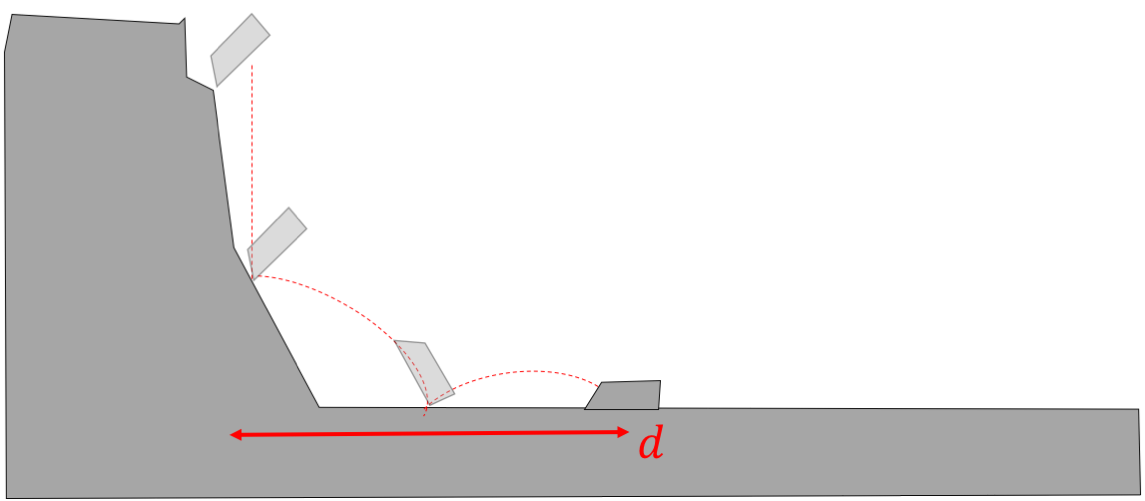
\includegraphics[width=0.7\textwidth]{images/distanza_frana}
	\caption{Rappresentazione di una frana di crollo. Il masso si stacca sulla cima del pendio e scende già aumentando la sua energia meccanica. Finito il pendio l'energia meccanica accumulata diminuisce fino ad esaurirsi. Il punto esatto dove si ferma il masso non è dato saperlo, ma si può stimare una distanza d oltre la quale ragionevolmente il masso non potrà spingersi.}
	\label{distanzaFrana}
\end{figure}

Un'altra osservazione la si può dedurre analizzando le fotografie scattate nei luoghi dove si sono verificate delle frane. In molti casi, soprattutto nei casi di frana da colamento, il terreno movimentato segue una traiettoria ben precisa (Figura \ref{traiettoriaFrana}). Quest'ultima dipende dalla morfologia del pendio, ovvero da come sono distribuite le masse di terreno lungo la discesa. Anche in questo caso è possibile stabilire un raggio d'azione inteso come la larghezza del "corridoio" dentro il quale la frana scivola (Figura \ref{traiettoriaFrana2}). Infine bisogna sempre tenere a mente che la forza di gravità è il fattore scatenante per eccellenza della frana, motivo per cui la pendenza del terreno giocherà sempre un ruolo fondamentale.

\begin{figure}[h]
	\centering
	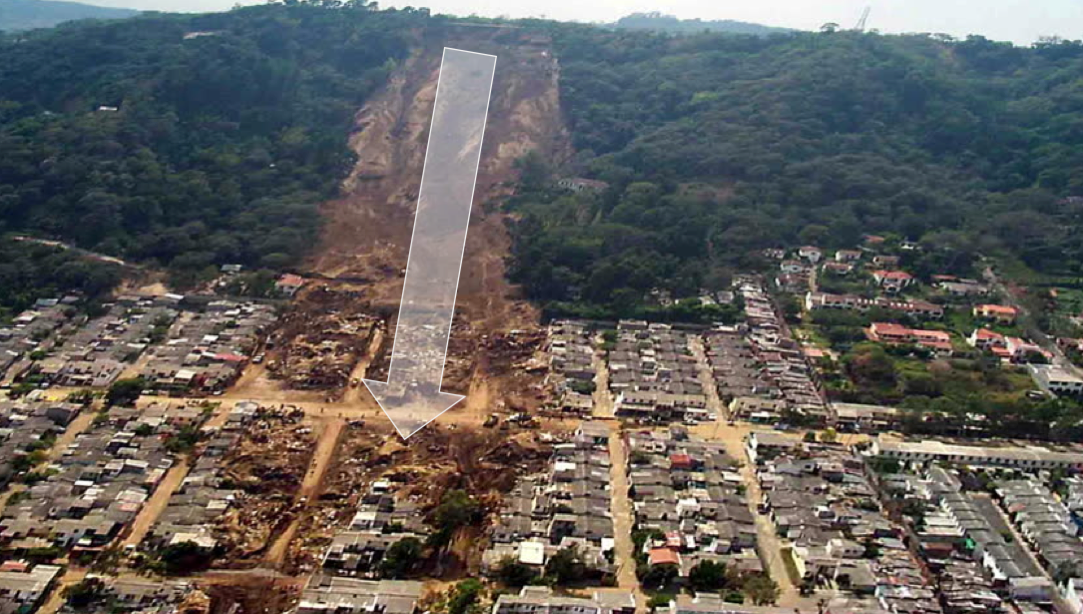
\includegraphics[width=0.7\textwidth]{images/traiettoria_frana}
	\caption{Frana di Colonia Las Colinas, El Salvador, 2001. E' possibile osservare come, in questo caso, la frana ha seguito una traiettoria ben delimitata tipica delle frane di colata. In questo caso specifico la distanza percorsa dalla frana è stata pari a circa 700 metri \textcolor{red} {(URL!!!!!!!!!!!!)}.}
	\label{traiettoriaFrana}
\end{figure}


\begin{figure}[h]
	\centering
	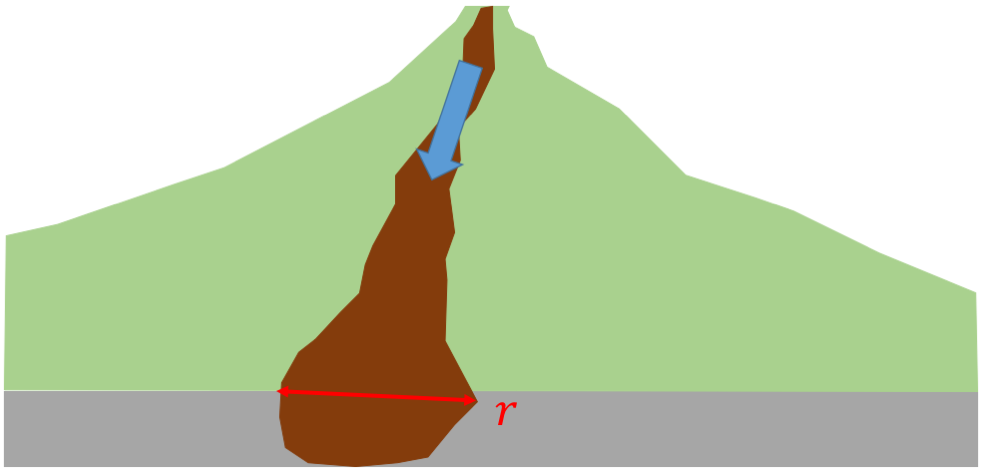
\includegraphics[width=0.7\textwidth]{images/traiettoria_frana2}
	\caption{Rappresentazione di una frana di colamento. E' possibile definire un raggio di azione r inteso come l'ampiezza del "corridoio" della frana.}
	\label{traiettoriaFrana2}
\end{figure}

La caratterizzazione di una frana è fondamentale e propedeutica ad enucleare una efficace strategia di prevenzione. Poter disporre di una strategia di questo tipo è particolarmente rilevante nel caso in cui l'ente che la mette in pratica ha un numero di \textit{assets strategici} molto elevato. Prendiamo in considerazione, solo per citare un esempio, Ferrovie dello Stato Italiane Spa. L'azienda possiede, tra i suoi assets, una rete ferroviaria di 16734 Km e più di 3,000 stazioni dislocate su un territorio (L'Italia) la cui superficie è di 301,340 $Km^2$. E' impensabile che i vertici delle Ferrovie dello Stato approvino un piano aziendale di prevenzione che preveda il controllo di ciascuna stazione e ciascun Km della rete ferroviaria! Sarebbe impossibile sia in termini di tempo necessario che di sforzo economico che l'Ente dovrebbe sostenere. 

La soluzione ideale sarebbe quella di avere un metodo che prenda in input un insieme di assets strategici e restituisca come output un lista ordinata in base alla loro esposizione al rischio frana. In questo modo sarebbe possibile occuparsi degli assets che sono veramente a rischio e quindi, oltre a risparmiare denaro, essere più rapidi negli interventi.

Il metodo da noi proposto verrà illustrato nelle prossime sezioni del documento. In particolare nella sezione 2 vengono fornite le definizioni dei concetti base, fondamentale per la comprensione del metodo, attraverso una formulazione matematica. Nella sezione 3 verrà spiegato in che modo le considerazioni fatte sulla pendenza del terreno e le traiettorie delle frane sono state affrontate e tradotte in equazioni matematiche. Infine nella sezione 4 verrà esposto come tali equazioni vengono utilizzate nello pseudo-codice dell'algoritmo.
